\documentclass[xcolor={dvipsnames}]{beamer}
%\usepackage[utf8]{inputenc}
\usetheme{CambridgeUS}

%-------------------------------------------------------------------------------
%          -Packages nécessaires pour écrire en Français et en UTF8-
%-------------------------------------------------------------------------------
\usepackage[utf8]{inputenc}
\usepackage[frenchb]{babel}
\usepackage[T1]{fontenc}
\usepackage{lmodern}
\usepackage{textcomp}

%-------------------------------------------------------------------------------

%-------------------------------------------------------------------------------
%                          -Outils de mise en forme-
%-------------------------------------------------------------------------------
\usepackage{hyperref}
\hypersetup{pdfstartview=XYZ}
\usepackage{enumerate}
\usepackage{graphicx}
%\usepackage{multicol}
%\usepackage{tabularx}

%\usepackage{anysize} %%pour pouvoir mettre les marges qu'on veut
%\marginsize{2.5cm}{2.5cm}{2.5cm}{2.5cm}

\usepackage{indentfirst} %%pour que les premier paragraphes soient aussi indentés
\usepackage{verbatim}
%\usepackage[table]{xcolor}  
%\usepackage{multirow}
\usepackage{ulem}
%-------------------------------------------------------------------------------


%-------------------------------------------------------------------------------
%                  -Nécessaires pour écrire des mathématiques-
%-------------------------------------------------------------------------------
\usepackage{amsfonts}
\usepackage{amssymb}
\usepackage{amsmath}
\usepackage{amsthm}
\usepackage{tikz}
\usepackage{xlop}
\usepackage[output-decimal-marker={,}]{siunitx}
%-------------------------------------------------------------------------------


%-------------------------------------------------------------------------------
%                    - Mise en forme 
%-------------------------------------------------------------------------------

\newcommand{\bu}[1]{\underline{\textbf{#1}}}


\usepackage{ifthen}


\newcommand{\ifTrue}[2]{\ifthenelse{\equal{#1}{true}}{#2}{$\qquad \qquad$}}

\newcommand{\kword}[1]{\textcolor{red}{\underline{#1}}}


%-------------------------------------------------------------------------------



%-------------------------------------------------------------------------------
%                    - Racourcis d'écriture -
%-------------------------------------------------------------------------------

% Angles orientés (couples de vecteurs)
\newcommand{\aopp}[2]{(\vec{#1}, \vec{#2})} %Les deuc vecteurs sont positifs
\newcommand{\aopn}[2]{(\vec{#1}, -\vec{#2})} %Le second vecteur est négatif
\newcommand{\aonp}[2]{(-\vec{#1}, \vec{#2})} %Le premier vecteur est négatif
\newcommand{\aonn}[2]{(-\vec{#1}, -\vec{#2})} %Les deux vecteurs sont négatifs

%Ensembles mathématiques
\newcommand{\naturels}{\mathbb{N}} %Nombres naturels
\newcommand{\relatifs}{\mathbb{Z}} %Nombres relatifs
\newcommand{\rationnels}{\mathbb{Q}} %Nombres rationnels
\newcommand{\reels}{\mathbb{R}} %Nombres réels
\newcommand{\complexes}{\mathbb{C}} %Nombres complexes


%Intégration des parenthèses aux cosinus
\newcommand{\cosP}[1]{\cos\left(#1\right)}
\newcommand{\sinP}[1]{\sin\left(#1\right)}

%Fractions
\newcommand{\myfrac}[2]{{\LARGE $\frac{#1}{#2}$}}

%Vocabulaire courrant
\newcommand{\cad}{c'est-à-dire}

%Droites
\newcommand{\dte}[1]{droite $(#1)$}
\newcommand{\fig}[1]{figure $#1$}
\newcommand{\sym}{symétrique}
\newcommand{\syms}{symétriques}
\newcommand{\asym}{axe de symétrie}
\newcommand{\asyms}{axes de symétrie}
\newcommand{\seg}[1]{$[#1]$}
\newcommand{\monAngle}[1]{$\widehat{#1}$}
\newcommand{\bissec}{bissectrice}
\newcommand{\mediat}{médiatrice}
\newcommand{\ddte}[1]{$[#1)$}

%Figures
\newcommand{\para}{parallélogramme}
\newcommand{\paras}{parallélogrammes}
\newcommand{\myquad}{quadrilatère}
\newcommand{\myquads}{quadrilatères}
\newcommand{\co}{côtés opposés}
\newcommand{\diag}{diagonale}
\newcommand{\diags}{diagonales}
\newcommand{\supp}{supplémentaires}
\newcommand{\car}{carré}
\newcommand{\cars}{carrés}
\newcommand{\rect}{rectangle}
\newcommand{\rects}{rectangles}
\newcommand{\los}{losange}
\newcommand{\loss}{losanges}


%----------------------------------------------------


\usepackage{../../pas-math}
\usepackage{../../moncours_beamer}


\graphicspath{{./img/}}

\title{Introduction à la cryptologie}
\author{O. FINOT}\institute{Lycée S$^t$ Vincent de Paul}


\AtBeginSection[]
{
	\begin{frame}
		\frametitle{Sommaire}
		\tableofcontents[currentsection, hideallsubsections]
	\end{frame} 
}


\AtBeginSubsection[]
{
	\begin{frame}
		\frametitle{Sommaire}
		\tableofcontents[currentsection, currentsubsection]
	\end{frame} 
}

\begin{document}



\begin{frame}
  \titlepage 
\end{frame}

\section{Introduction}

\begin{frame}
\frametitle{Introduction}	
	
	\begin{block}{Historique}
		\begin{itemize}
			\item Utilisé depuis toujours
			\item Cacher, dissimuler des informations essentielles / confidentielles\pause
			\item[$\Rightarrow$] Cryptologie
		\end{itemize}	\pause
	\end{block}
	
	\begin{block}{Aujourd'hui : Sur internet}
		\begin{itemize}
			\item Informations confidentielles
			\item Impôts
			\item Paiements en ligne\pause
			\item[$\Rightarrow$] Données ne doivent pas circuler "en clair"
		\end{itemize}
	\end{block}
	
\end{frame}

\begin{frame}
	\frametitle{Sommaire}
	\tableofcontents[hideallsubsections]
\end{frame} 

\section{Vocabulaire}

\begin{frame}
\frametitle{Définitions I}


	\begin{alertblock}{Cryptologie}
		\begin{itemize}
			\item Science des messages secrets
			\item Cryptographie vs. Cryptanalyse
		\end{itemize}
	\end{alertblock}\pause
	
	\begin{block}{Cryptographie}
		"Art" de transformer un message pour le rendre illisible
	\end{block}\pause
	
	\begin{block}{Cryptananlyse}
		"Art" de rendre un message transformé lisible
	\end{block}
\end{frame}

\begin{frame}
\frametitle{Définitions II}	

	\begin{block}{Chiffrer / Crypter}
		Transformer un message
	\end{block}\pause
	
	\begin{block}{Décrypter}
		Rendre un message lisible
	\end{block}
	

\end{frame}
\section{Chiffrements par substitution monoalphabétique}

\subsection{Principe}

\begin{frame}
\frametitle{Principe des chiffrements par substitution}

\begin{itemize}
	\item Chaque lettre remplacée par une autre
	\item Toujours la même lettre d'arrivée pour une lettre donnée
\end{itemize}

\end{frame}


\subsection{Exemples}

\begin{frame}
\frametitle{Chiffre de César}
\framesubtitle{Présentation}

\begin{block}{Historique}
	\begin{itemize}
		\item Utilisé par César 
		\item Transmission des ordres à ses généraux 
	\end{itemize}
	\end{block}
	
	\begin{block}{Principe}
		\begin{itemize}
			\item Choix d'une distance (26 possibilités)
			\item Remplacement d'une lettre par celle qui se trouve à la distance choisie   
		\end{itemize}
		
		\begin{center}
			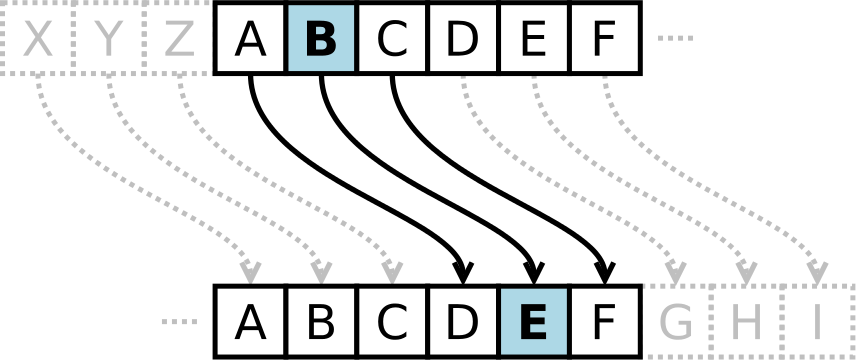
\includegraphics[scale=0.2]{cesar}			
		\end{center}

	\end{block}
	
\end{frame}




\begin{frame}
\frametitle{Chiffre de césar}
\framesubtitle{Exemple avec une distance de 3}


	\begin{center}
		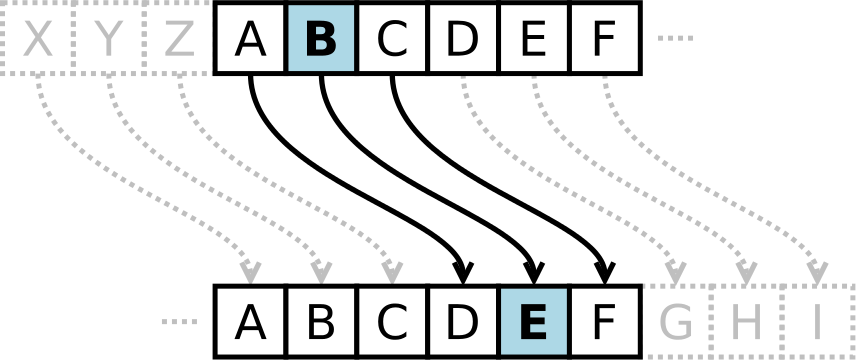
\includegraphics[scale=0.2]{cesar}			
	\end{center}

\begin{itemize}
	\item ALEA JACTA EST\pause
	\item[$\Rightarrow$] DOHD MDFWD HVW
\end{itemize}


\end{frame}


\begin{frame}
	\frametitle{Substitution "aléatoire"}
	
	\begin{block}{Principe}
		\begin{itemize}
			\item Pas de distance fixe
			\item Choix d'une lettre de remplacement pour chaque lettre d'origine
		\end{itemize}
	\end{block}
	
	\begin{exampleblock}{Exemple de substitution}
		\begin{itemize}
			\item ABCDEFGHIJKLMNOPQRSTUVWXYZ
			\item AZERTYUIOPQSDFGHJKLMWXCVBN\pause
			\item []
			\item[$\Rightarrow$] SUBSTITUTION devient LWZLMOMWMOGF
		\end{itemize}
		
		
	\end{exampleblock}
	
	
\end{frame}


\subsection{Bilan}

\begin{frame}
\frametitle{Décryptage}

\begin{block}{Analyse fréquentielle}
	\begin{itemize}
		\item Repérer les lettres qui apparaissent le plus
		\item En français : E
	\end{itemize}
\end{block}

\begin{center}
	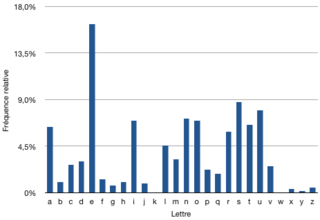
\includegraphics[scale=0.6]{freq}\footnote{Source wikipédia}
\end{center}	

\end{frame}

\begin{frame}
\frametitle{Avantages / Inconvénients}

\begin{exampleblock}{Avantages}
	\begin{itemize}
		\item Faciles à comprendre
		\item Faciles à utiliser
	\end{itemize}
\end{exampleblock}

\begin{alertblock}{Incovénients}
	\begin{itemize}
		\item Faciles à casser
	\end{itemize}
\end{alertblock}
\end{frame}
\section{Chiffrements par clé}

\subsection{Chiffrements symétriques}

\begin{frame}
\frametitle{Principe du chiffrement symétrique}

\begin{itemize}
	\item Une clé pour chiffrer un message
	\item La même pour décrypter
\end{itemize}

\begin{center}
	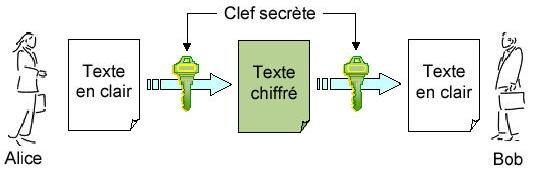
\includegraphics[scale=0.5]{sym}
\end{center}
\end{frame}

\begin{frame}
\frametitle{Chiffre de Vigénère}

\begin{block}{Principe}
	\begin{itemize}
		\item Choix d'une clé
		\item Correspondance entre le texte en clair et la clé
	\end{itemize}
	
	\begin{center}
		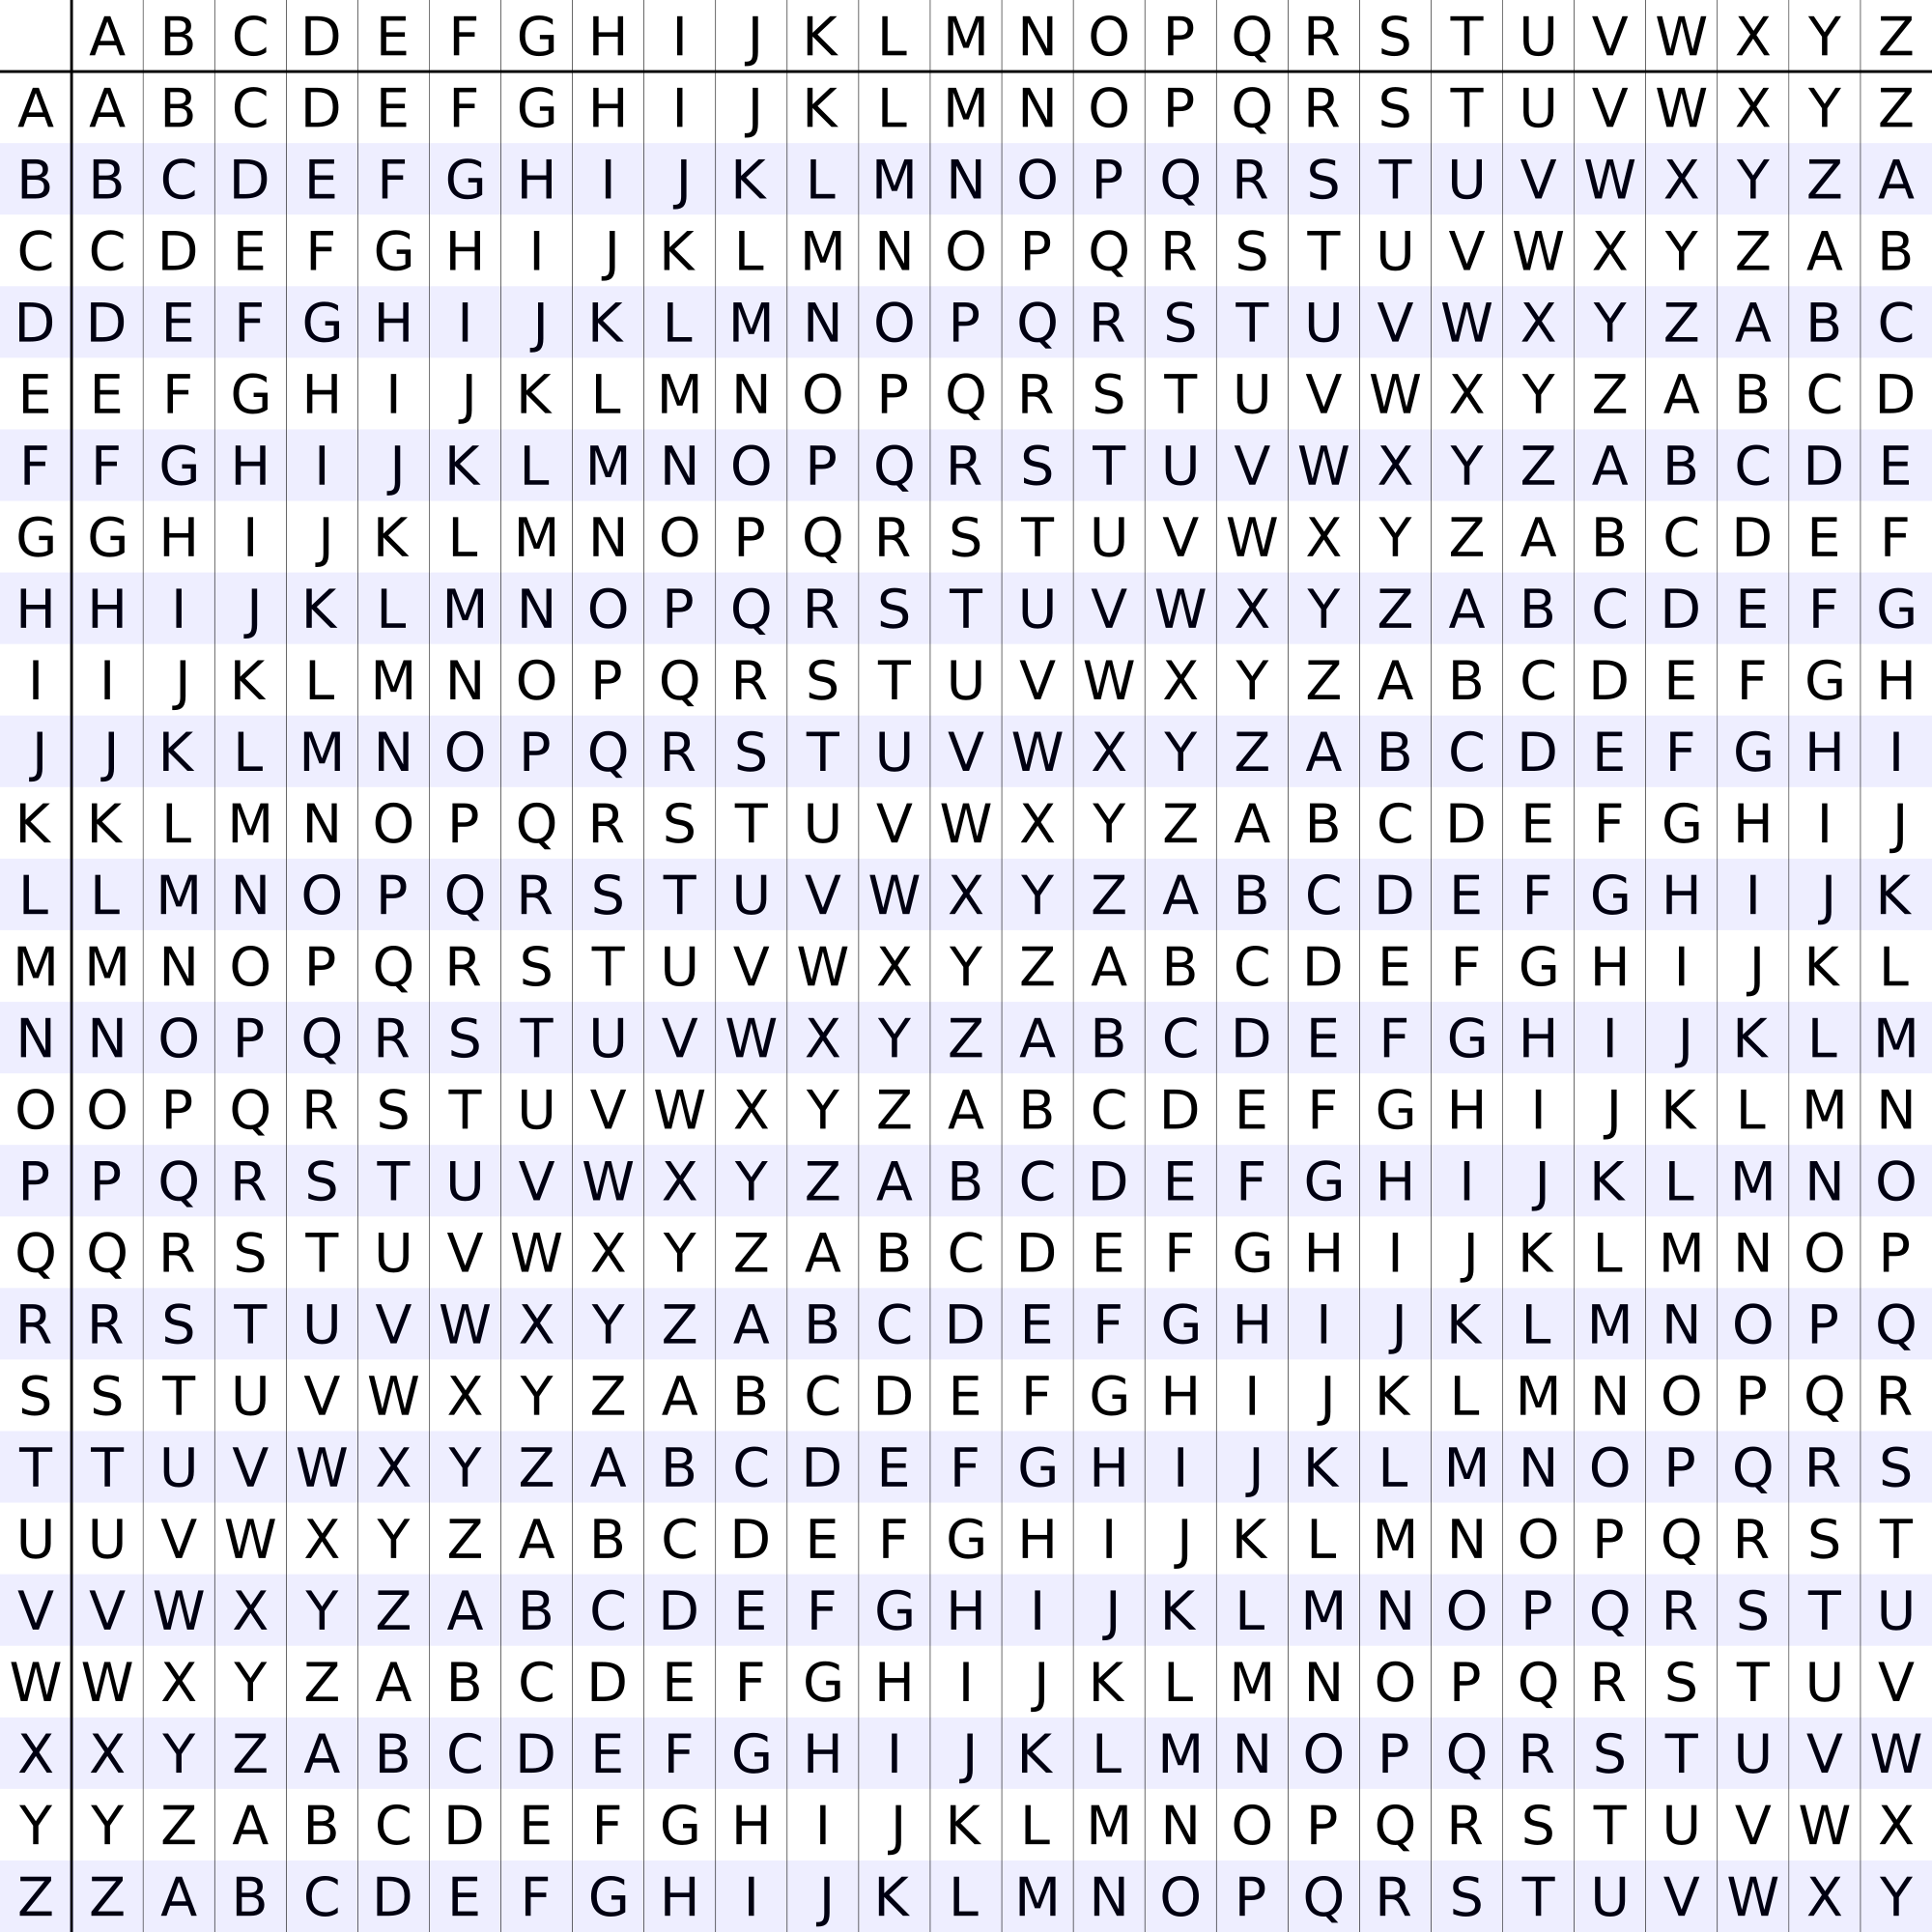
\includegraphics[scale=0.08]{vigenere}
	\end{center}
\end{block}
\end{frame}

\begin{frame}
	\frametitle{Bilan}
	
	\begin{exampleblock}{Avantage}
		\begin{itemize}
			\item Très sûr (si clé assez longue)			
		\end{itemize}
	\end{exampleblock}
	
	\begin{alertblock}{Inconvénient}
		\begin{itemize}
			\item \'Echange de la clé
		\end{itemize}
	\end{alertblock}
	
\end{frame}

\subsection{Chiffrements Asymétriques}

\begin{frame}
	\frametitle{Principe du chiffrement asymétrique}
	
	\begin{block}{Principe}
	
		\begin{itemize}
			\item 2 clés
			\item 1 clé publique distribuée à tout le monde
			\item 1 clé privée gardée pour soi
		\end{itemize}
	\end{block}
	
	\begin{center}
		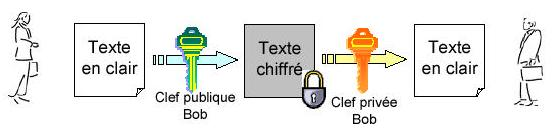
\includegraphics[scale=0.5]{asym}
	\end{center}	
	
\end{frame}

\section{Conclusion}


%\begin{columns}[c]
%	\begin{column}{6cm}
%		\begin{itemize}
%			\item $f(x)=2x$
%			\item $g(x)=-x+2$
%		\end{itemize}
%	\end{column}
%	\begin{column}{6cm}
%		\begin{itemize}
%			\item $h(x)=3x-4$
%			\item $i(x)=5$
%		\end{itemize}
%	\end{column}				
%\end{columns}



\end{document}